\section{METHOD}
\label{chap:method}
We already defined an attack graph. We, now, look at how the existing components of attack graph generation for computer networks map into a microservice environment, we illustrate the concepts using a small example in Subsection \ref{chap:mapping}. We then, in Subsection \ref{chap:technical}, present the tools that we use to achieve this mapping and present an overview of our proposed system and its components: Topology Parser in Subsection \ref{chap:topology_p}, Vulnerability Parser in Subsection \ref{chap:vulnerability_p} and Attack Graph Parser Subsection \ref{chap:attack_graph_p} with the Breath-first Search graph traversal algorithm in Subsection \ref{chap:bfs}. 


\subsection{From Network Nodes to Microservices}
\label{chap:mapping}
% abit reptative 
In our work, we adapt already existing attack graph generation methods from computer networks to the microservices ecosystem. In order to do this, we identify the different components and find a compatible replacement that can be used in a microservice architecture. In this subsection, we start first by shortly introducing a famous framework (Docker) and some of its terminology. We then modify the attack graph concepts mentioned in Subsection \ref{chap:attack_graphs}: nodes, edges, privilege levels, pre- and postconditions to match our use-case. We illustrate the whole idea  by demonstrating a small example.

Docker is one of the most popular and used containerization frameworks currently available. In Docker, a distinction is being made between the terms \textit{image}, \textit{container} and \textit{service}. An \textit{image} is an executable package that includes everything needed to run an application, a \textit{container} is a runtime instance of an image, and a \textit{service} represents a container in production. A service only runs one image, but it codifies the way that image runs, what ports it should use, how many replicas of the container should run so the service has the capacity it needs \cite{merkel2014docker}. In our work, we construct attack graphs by statically analyzing the topology of the containers, hence, we treat these terms equally.  

Privileges play a central role in the generation if attack graphs. Traditionally, the privileges are modeled as a hierarchy that varies in the access level (\textit{User, Admin}), and the access scope (virtual machine VOS, host machine OS). The exhaustive list of privileges, that are used in this paper, are: \textit{None, VOS(User), VOS(Admin), OS(User) and OS(Admin)}. VOS means that the privilege is exclusive to a virtual machine, while not affecting the host machine. However in our case, unlike hosts connected in a computer network, these privileges refer to images and not virtual machines. On the other side, the keyword \textit{OS} means that the  host machine can be controlled by a user who has this privilege. Since \textit{VOS} are isolated from host machines and their exploitation does not imply the exploitation of the host machine, they are in the lower level of the hierarchy \cite{aksu2018automated}. \textit{None} means that no privilege is obtained, \textit{User} means only a subset of user level privileges are granted, and \textit{Admin} grants control over the whole system.

As mentioned earlier, the \textit{nodes} and the \textit{edges} are the basic building blocks of an attack graph. A \textit{node} represents  a combination of a docker image and its respective compromise levels (expressed as privileges obtained by the attacker). A directed \textit{edge} between two nodes represents an attack step from one node (a compromised image with a certain privilege gained by the attacker) to another node (adjacent exploitable image with the gained privileges). Each edge is typed with the vulnerability (CVE) that could be exploited in the end node.

In order for attackers to exploit a given vulnerability, they need to have certain \textit{preconditions}, i.e, the minimum privileges needed to exploit \cite{aksu2018automated}. Once an attacker meets these preconditions and exploits the vulnerability, he gains the privilege of the end node as a \textit{postcondition} and a directed edge is added between them. Both the pre- and postconditions in this work are transformed from pre- and postcondition rules manually selected and evaluated by experts in existing work \cite{aksu2018automated}. The pre- and postcondition rules use the fields defined by NVD, as well as an occurrence of specific keywords from the CVEs descriptions \cite{booth2013national}.

\subsubsection{Example}

\begin{figure*}[!h]
	\centering
	\begin{subfigure}[b]{\columnwidth}
		\centering
		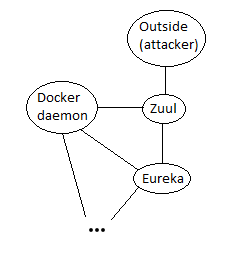
\includegraphics[width=.5\linewidth]{./images/Topology_graph}
		\caption{}
		\label{TopologyGraph}
	\end{subfigure}
	\hfill
	\begin{subfigure}[b]{\columnwidth}
		\centering
		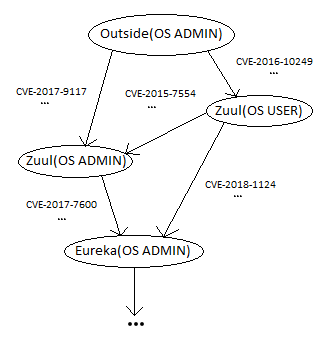
\includegraphics[width=.5\linewidth]{./images/Attack_graph}
		\caption{}
		\label{AttackGraph}
	\end{subfigure}
	
	\caption[Two numerical solutions]{Reduced Netflix OSS example (a) Example topology graph  (b) Example resulting attack graph}
\end{figure*}


In order to show how the attack graph generation works in practice, we present a small example. The example is taken from the Netflix OSS Github repository. Netflix OSS example is a Spring Cloud-based microservices architecture that uses the following microservices: Service Discovery (Eureka), Circuit Breaker (Hystrix), Intelligent Routing (Zuul) and Client Side Load Balancing (Ribbon) \cite{netflixoss, springcloudnetflix}. Displayed in Figure \ref{TopologyGraph} is a subset of the example topology where each node denotes a container and each edge is a connection between two containers, if one calls the other. The topology consists of an "Outside" node, "Docker daemon" node, Zuul, Eureka and other nodes. According to Netflix, Zuul is an edge service that provides dynamic routing, monitoring, resiliency, and security functionalities. Eureka is a REST (Representational State Transfer) based service that is primarily used in the cloud for locating services for the purpose of load balancing and fail-over of middle-tier servers. In Figure \ref{AttackGraph} we can see a part of the corresponding attack graph, where a node is a pair of the image and its privilege, while an edge represents an atomic attack. Parts of both graphs have been intentionally omitted to reduce complexity. An example path that an attacker would take could be to first attack the Zuul container by exploiting the CVE-2016-10249 vulnerability by crafting an image file, which triggers a heap-based buffer overflow\footnote{\url{https://nvd.nist.gov/vuln/detail/CVE-2016-10249}} and gain USER privilege.  With this USER privilege, an attacker can exploit the CVE-2015-7554 vulnerability on the same container via crafted field data in an extension tag in a TIFF image\footnote{\url{https://nvd.nist.gov/vuln/detail/CVE-2015-7554}} to gain ADMIN privilege. Once the ADMIN privilege has been obtained on Zuul, the attacker can attack the Eureka container by exploiting CVE-2017-7600 via another crafted image\footnote{\url{https://nvd.nist.gov/vuln/detail/CVE-2017-7600}} and gain ADMIN privilege. It is important to note that this is not the only path that the attacker can take in order to have ADMIN privileges on Eureka. Another path would be to exploit the CVE-2018-1124 vulnerability via creating entries in procfs by starting processes, which could result in crashes or arbitrary code execution\footnote{\url{https://nvd.nist.gov/vuln/detail/CVE-2018-1124}}. This vulnerability can be exploited by having only USER privilege on Zuul to gain directly ADMIN privileges of the Eureka container. Our attack graph generator shows both paths since it is of an interest to see every possible route in which a container can be compromised.



\subsection{Attack Graph Generation for Docker Networks}
\label{chap:technical}

 Figure \ref{AttackGraphSystem} gives an overview of the attack graph generator. In the figure, the rectangles denote the main components of the system, while the arrows describe the flow of the system and the files are the intermediate products. Our attack graph generator is composed of three main components: \textit{Topology Parser, Vulnerability Parser and Attack Graph Generator}. The Topology Parser reads the underlying topology of the system and converts it into to a format needed for our Attack Graph Generator, the Vulnerability Parser scans the vulnerabilities for each of the images and the Attack Graph Parser generates the attack graph from the topology and vulnerabilities files. In the following subsections, we first have a look into the system requirements, then describe each component in more details.

The generator is developed and tested for Docker 17.12.1-ce and Docker Compose 1.19.0 \cite{merkel2014docker}. Docker Compose\footnote{\url{https://docs.docker.com/compose/}} is a tool for defining the orchestration of a multi-container applications. It provides a static configuration file that specifies the system containers, networks, and ports. Clair and ClairCtl \footnote{\url{https://github.com/coreos/clair}}  are used for vulnerabilities scanning. The generator is written in Python 3.6. Although we used  specific versions of the tools, the pipe and filter structure of the generator can be easily extended to other versions of Docker-Compose, vulnerability scanners and microservice architectures by replacing.


\textbf{TODO rename the attack graph parser in the box to Attack graph Generator}
\begin{figure}
	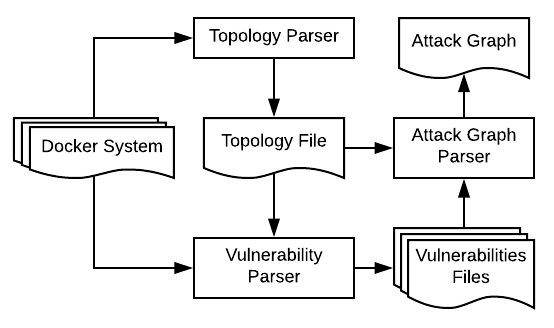
\includegraphics[scale=0.9]{./images/AttackGraphSystem}
	\caption{Overview of the Attack Graph Generator System}
	\label{AttackGraphSystem}
\end{figure}

\subsubsection{Topology Parser}
\label{chap:topology_p}

In order to generate an attack graph of a given system, we require an arrangement of its components and connections described as a system topology. The topology of Docker containers can be described either at  runtime or at design time by using Docker Compose. In our case, since we are doing static attack graph analysis, we use Docker Compose to extract the topology. Docker Compose provides a  file (docker-compose.yml) which is used for describes the orchestration of the services. However different versions of docker-compose.yml, use different syntax. For example, older versions use the deprecated keyword "\textit{link}", while newer ones use exclusively "\textit{networks}", to denote a connection between two images. In this work, we use the keyword "\textit{networks}" as an indicator that a connection between two images exists.

In the majority of cases, for an application to be useful, it communicates with the outside world, i.e, it has end points that can be used by the outer network. In Docker, this is usually done by using publishing ports. This is the case in both computer networks, as well as in microservice architectures.

Another consideration that we take into account is the \textit{privileged access} \footnote{\url{http://obrown.io/2016/02/15/privileged-containers.html}} \cite{libvirt}. Some containers obtain certain privileges that grant them control over the docker daemon in order to function properly. For example, a user may want to run some hardware (e.g., web-cam) or some applications that demand higher privilege levels  from Docker. In Docker, this is usually done either by mounting the Docker socket or specifying the keyword "privileged" in the docker-compose.yml file. An attacker with access to these containers has also access to the Docker daemon. Once the attacker has access to the Docker daemon, he has potential access to the whole microservice system, since every container is controlled and hosted by the daemon.




\subsubsection{Vulnerability Parser}
\label{chap:vulnerability_p}

In the preprocessing step, we use Clair to generate the vulnerabilities of a given image. Clair is a vulnerability scanner that inspects a Docker image and generates its vulnerabilities by providing \textit{CVE-ID}, a description and attack vector for each vulnerability. An attack vector is an entity that describes which conditions and effects are connected to this vulnerability. We collect the fields in the attack vector which are,  as described by the National Vulnerability Database(NVD) \cite{booth2013national}, Access Vector (Local, Adjacent Network and Network), Access Complexity (Low, Medium, High), Authentication (None, Single, Multiple), Confidentiality Impact (None, Partial, Complete), Integrity Impact (None, Partial, Complete) and Availability Impact (None Partial, Complete). Unfortunately, Clair does not provide a command line interface to analyze a docker image. We use another tool, i.e.,  Clairctl  to analyze a complete docker image.

\begin{algorithm}
	\SetAlgoLined
	\KwData{topology, cont\_expl,
		priv\_acc}
	\KwResult{nodes, edges}
	nodes, edges, passed\_nodes = [], [], [] \\
	queue = Queue() \\
	queue.put("outside" + "ADMIN") \\
	
	\While{! queue.isEmpty()}{
		curr\_node = queue.get() \\
		curr\_cont = get\_cont(curr\_node) \\
		curr\_priv = get\_priv(curr\_node) \\
		neighbours = topology[curr\_cont] \\
		\For{neigh in neighbours}{
			\If{curr\_cont == docker\_host}
			{
				end = neigh + "ADMIN" \\
				create\_edge(curr\_node, end) \\
			}
			\If{neigh == docker\_host and priv\_acc[curr\_cont]}
			{     
				end = neigh + "ADMIN" \\
				create\_edge(curr\_node, end) \\
				queue.put(end) \\
				passed\_nodes.add(end)        
			}
			\If{neigh != outside and neigh != docker\_host}{
				precond = cont\_expl[neigh][precond] \\
				postcond = cont\_expl[neigh][postcond] \\
				\For{vul in vuls}{
					\If{$curr_priv > precond[vul]$}{    
						end = neigh + post\_cond[vul]\\
						create\_edge(curr\_node, end\_node)\\
						\If{end\_node not in passed\_nodes}{
							queue.put(end\_node)\\
							passed\_nodes.add(end\_node)
					}}
				}
			}
		}
		nodes = update\_nodes()\\
		edges = update\_edges() \\
	}
	
	\caption{BFS algorithm for attack graph generation}
	\label{BFSalgorithm}
\end{algorithm}

\subsubsection{Attack Graph Generator}
\label{chap:attack_graph_p}

After the topology  is extracted and the vulnerabilities for each container are generated, we continue with the attack graph generation. Here, we first pre-process the vulnerabilities and convert them into sets of pre- and postconditions. In order to do this, we match the attack vectors acquired earlier from the vulnerability database and keywords of the descriptions of each vulnerability to generate attack rules. When a subset of attack vector fields and description keywords matches a given rule, we use the pre- or postcondition of that rule. If more than one rule matches, we take the one with the highest privilege level for the preconditions and the lowest privilege level for the postconditions. If no rule matches, we take None as a precondition and ADMIN(OS) as a postcondition. This results in a list of container vulnerabilities with their preconditions and postconditions. \textbf{TODO give an example of the attack rule and refer to the source of these rules}

\paragraph{Breadth-first Search}
\label{chap:bfs}

After the preprocessing step is done, the vulnerabilities are parsed and their pre- and postconditions are extracted. Together with the topology, they are feed into a Breadth-first Search algorithm (BFS).
Breadth-first Search is a popular search algorithm that traverses a graph by looking first at the neighbors of a given node, before diving deeper into the graph. A pseudo-code of our modified Breadth-first Search is given in Algorithm \ref{BFSalgorithm}. The algorithm requires a topology and a dictionary of the exploitable vulnerabilities as an input and the output is made up of nodes and edges that make the attack graph \textbf{TODO please explain what is cont expl, priv acc and refer to them in the text}. The algorithm first initializes the nodes, edges, queue and the passed nodes. Afterward, it generates the nodes which are a combination of the image name and the privilege level. Then into a while loop, it iterates through every node, checks its neighbors and adds the edges if the conditions are satisfied. If the neighbor was not passed, then it is added to the queue. The algorithm terminates when the queue is empty. Furthermore, BFS is characterized by the following properties.
\textbf{TODO: add line numbers to the algo and refer to those numbers in the text.}


\begin{itemize}
	\item Completeness: Breadth-first Search is complete i.e. if there is a solution, Breadth-first search will find it regardless of the kind of graph.
	\item Termination: This follows from the monotonicity property. Monotonicity is ensured if it is assumed that an attacker will never need to relinquish a state \cite{ingols2006practical, ou2006scalable, ammann2002scalable}. In this implementation, each edge is traversed only once, making sure that monotonicity is preserved.
	\item  Complexity: is $O(|N| + |E|)$ where $|N|$ is the number of nodes and $|E|$ is the number of edges in the attack graph.
\end{itemize}


